% -------------
% DO NOT DELETE.
% DO NOT DELETE.
% DO NOT DELETE.
% -------------
Every correct node is chosen by the scheduler at most a fixed number of times, $\delta$, after which the value of every correct node is collected and counted.
Note another (and final) condition: if a node is selected and that node has seen $\phi$ consecutive majorities for the same value, it no longer updates its value, regardless of the output of the polling. 

\subsubsection{Safety of \Theta_1}
The expression for the hypergeometric experiment is reasonably complex, and it becomes hard to reason about the different ways that each of the variables inside the expression affects the outcomes. In particular, it is not clear how network size affects the experiment. This is of interest because if the effect of network size has little bearing on the outcomes of the experiment, it has important consequences for the scalability of the $\Theta_1$ protocol. To see how network size affects the system, we can fortunately make usage of the 

\subsubsection{Adversarial Optimality}
We will first try to determine the optimal strategy that the Byzantine
adversary can play.  Once we have this strategy, we will analyze how
effective this strategy is.
Recall that we do not care about violating liveness for conflicting
transactions, so the adversary's objective is to violate
safety, that is, it wants some correct node to decide red while another
correct node decides blue.  

As a thought experiment, consider that most correct nodes lean red
while only one correct node leans blue.  Given our sampling protocol,
it is clear that if there are not too many Byzantine nodes, the red-leaning
nodes will continue to lean red, while the blue-leaning node will
start increasing its confidence in red and eventually become red-leaning
as well.  It thus stand to reason that a primary objective of the adversary
is to have half of the correct nodes lean red, while the other half lean
blue, and to keep it this way.

However, the adversary faces a conflict.  Consider that the adversary
has only limited time ($\phi$ rounds) to accomplish its goal of
violating safety.  When half the nodes are leaning blue, and half
the nodes are leaning red, their confidence in either blue or red
will not grow rapidly, and they likely will not decide in the limited
amount of time.  Also, if some node $u$ is close to deciding blue
and a small majority of nodes are leaning blue, then if $u$ polls
a Byzantine node it is not clear whether the Byzantine node should
return red or blue.  If the Byzantine node returns blue, it may
cause $u$ to decide blue but still give the adversary a chance to
get other nodes to decide red.  If the Byzantine node returns red,
it may help restore the balance between red- and blue-leaning nodes.

This conflict for the adversary illustrates exactly the strength of
the Snowball protocol.  While it is relatively easy for the adversary
to prevent deciding on conflicting transactions, it is difficult for
the adversary to cause two correct nodes to decide different transactions.

\begin{comment}
If this is the situation, then if a correct
node samples other nodes, it will, by expectation, receive the same number of
red and blue votes from the correct nodes that it samples.

The Byzantine strategy then is straightforward:
if there are as many red-leaning nodes as blue-leaning nodes and
a red-leaning node samples from a Byzantine node, the Byzantine node
returns red, and vice versa.
If the node has equal confidence in red or blue, it does not matter
which color the Byzantine node returns and can, say, flip a coin.
If, however, the system is not in balance, and
there are more red than blue nodes, then a Byzantine node will always
``push back'' by returning blue (and vice versa).
We will later demonstrate that this strategy is optimal.

Next, we need to show that although optimal, the strategy cannot
cause a violation of safety with high probability.
We will show that whp no 
correct node ever decides (if there are conflicting values), and in particular
no two correct nodes ever disagree.
If the Byzantine strategy is non-optimal, correct nodes may decide, but
they will decide the same value whp.
\end{comment}

\begin{comment}
We define \emph{skew} as the maximum among the distances between the
confidence vectors (interpreted as points in a Euclidean space)
of correct node pairs.  For example, if there are three correct nodes
with confidence vectors $\langle 0, 3 \rangle$, $\langle 1, 3 \rangle$,
and $\langle 4, 0 \rangle$, then the skew is~5 (the distance between
the first and last confidence vector endpoints).
The optimal strategy for the Byzantine nodes is to maximize skew.

% TODO: Expand in sentences the notation written about maximal policy below. 
We want to characterize \textit{drift} in the differences of values between any two correct nodes. Specifically, letting the absolute difference between the values of any correct node correspond to some confidence differential, represented by $\max_{\Delta}(u) = u[0]-u[1]$ if $|u[0]| > u[1]$ and $\max_{\Delta}(u) = u[1]-u[0]$ if $u[1] > |u[0]|$, we desire to precisely quantify bounds on the maximum drifts between any two correct nodes, and for all possible execution instances $\mathcal{I}_i$. In other words, what is the execution path $\mathcal{I}_{opt}$ such that
\[
    \mathcal{I}_{opt}(\mathcal{C}^{t_0}) = \max_{\forall i}\{\mathcal{I}_i(\mathcal{C}^{t_0})\}
\]
where
\[
    \mathcal{I}_{i}(\mathcal{C}^{t_0}) = \max_{\forall u, v \in \mathcal{C}^{t_\phi}}\{\max_{\Delta}(u)-\max_{\Delta}(v)\}
\]
To exactly characterize the probability of a safety failure of the optimal execution path, we would need to calculate the probability distribution over all possible permutations of Byzantine answers, which is a function of the choices of execution of the correct nodes as well as the distribution of the choices of the neighbors.
In other words, over all possible execution paths (i.e. there are $c$ nodes to choose at each time step, for a total of $\phi^{c}$ ways of choosing over $\mathcal{C}$ nodes) and over all possible choices of the $k$-sampled neighbors (for a total of ${n \choose k}$ such choices, per node, per execution round), we would need to keep track of all of the possible tuples of the Byzantine value updates. 
Generating such a stochastic model would, plainly speaking, be infeasible. 
\end{comment}

\paragraph{Optimality Condition}
We can simplify the analysis greatly if we fix the Byzantine strategy to some optimal policy, $\mathcal{A}_{\pi}$. 
Let $s$ be a three-tuple where the first entry is a color configuration of the set of nodes in $\mathcal{C}$ (i.e. the set $\lbrace(u_1[\mathtt{R}], u_1[\mathtt{B}]), (u_2[\mathtt{R}], u_2[\mathtt{B}]), \dots, (u_c[\mathtt{R}], u_c[\mathtt{B}])\rbrace$, where $u[\mathtt{R}], u[\mathtt{B}] \in [0, \phi]$), the second entry is the chosen node at some round $u \in \mathcal{C}$ in round $t_i$, and the third entry is the round itself $t_i$. Let $\mathtt{S}$ be the set of all such tuples $s$. The elements of $\mathtt{S}$ are the necessary pieces of information needed for the Byzantine strategy. 
For each state $s \in \mathtt{S}$, the set of allowable actions for the Byzantine nodes is either $\mathtt{R}$ or $\mathtt{B}$. Let $P(s' | s, {\mathtt{R}})$ be the probability of transitioning from state $s$ to $s'$ given that the Byzantine strategy responds with $\mathtt{R}$, and conversely for $\mathtt{B}$. Let $\mathtt{Z}(s)$ be the reward for entering state $s$. Let the policy $\mathcal{A}_{opt}(s)$ be the optimal policy which returns the color chosen by the Byzantine node at state $s$, given round $i$. 
The utility $\mathcal{U}$ of $s$ (and the optimal policy) are then defined as
\begin{equation}
\begin{split}
\mathcal{U}(\mathcal{A}_{opt}, s) =\ \mathtt{Z}(s)\ +& \sum_{s' \in S} P(s' | s, \mathcal{A}_{opt}(s))\\
\times &\ \mathcal{U}(\mathcal{A}_{opt}, s')
\end{split}
\end{equation}
where 
\begin{equation}
\begin{split}
    \mathcal{A}_{opt}(s) &= \argmax_{a \in \lbrace \mathtt{R}, \mathtt{B} \rbrace} \left \lbrace \sum_{s' \in S}P(s'|s, a)\mathcal{U}(\mathcal{A}_{opt}, s') \right \rbrace
\end{split}
\end{equation}
These are the equations that follow from Bellman's optimality principle. Note that we do not include a discount factor. Further, we assign a reward of 1 to the states where there exists two nodes $u, v$ such that $\gamma_u \geq \gamma$ and $\gamma_v \leq 1/\gamma$. 

Since the state space is computationally infeasible, we solve for the optimal policy inductively, rather than iteratively. 
Let $count(\mathcal{C}^{t_i}, \mathtt{R})$ be defined as: 
\begin{equation}
\begin{split}
    count(\mathcal{C}^{t_i}, \mathtt{R}) = \sum_{u \in \mathcal{C}^{t_i}} \mathbbm{1}(u, \mathtt{R})
\end{split}
\end{equation}
where $\mathbbm{1}$ is the indicator function defined as:
\begin{equation}
\begin{cases}
    \mathbbm{1}(u, \mathtt{R}) = 1\ \text{\textbf{if}}\ u[\mathtt{R}] > u[\mathtt{B}]\\
    \mathbbm{1}(u, \mathtt{R}) = 0\ \text{\textbf{if}}\ u[\mathtt{R}] < u[\mathtt{B}]\\
    \mathbbm{1}(u, \mathtt{R}) = \{1, 0\}\ \text{\textbf{if}}\ u[\mathtt{R}] == u[\mathtt{B}]\ \text{\textbf{and} $u$ lastly}\\
    \text{preferred $\{\mathtt{R}, \mathtt{B}\}$}
\end{cases}
\end{equation}
and conversely for $count(t_i, \mathtt{B})$. 

Let $\mathcal{C}_{\mathtt{R}}$ be the set of correct nodes that the Byzantine nodes color as red at the cold start phase, and $\mathcal{C}_\mathtt{R}$ the converse. It is easy to see that a coloring of equal split between red and blue in the cold-start phase is the optimal configuration for a single iteration of the $\Theta_1$ protocol. It is not clear, however, how this configuration must evolve (if at all) as time progresses. 

Let $\mathcal{A}_\pi$ be the chosen Byzantine strategy described formally in Figure \ref{figure:mathcal_a_pi}. 
\begin{figure}[h!]
\label{figure:mathcal_a_pi}
\fbox{
    \parbox{0.95\linewidth}{
        \begin{center}
            \textbf{The $\mathcal{A}_\pi$ policy}
        \end{center}
        Let the Byzantine nodes set $\mathcal{C}_\mathtt{R}$ to be exactly half of the correct nodes in the network, and $\mathcal{C}_\mathtt{B}$ the other half at the cold-start phase. We initialize a local memory $\mathds{M}$, which stores various information about the history of execution up to step $t_i$. Let $\{\mathcal{C}', u, t_i\} \leftarrow s$, where $\mathcal{C}^{t_i} = \mathcal{C}'$ (note that there are multiple valid versions of $\mathcal{C}^{t_i}$, nevertheless in this case we refer to the specific set $\mathcal{C}$ extracted from state $s$). 
        \begin{itemize}
            \item If $count(\mathcal{C}^{t_i}, \mathtt{R}) = c/2$:
            \subitem In this case, the set of correct nodes is equally split. If $u \in \mathcal{C}_\mathtt{R}$, then all Byzantine nodes are colored red. Conversely for blue. Add $s$ to $\mathds{M}$, and return. 
            \item If $count(\mathcal{C}^{t_i}, \mathtt{R}) < c/2$:
            \subitem In this state, the set of correct nodes has shifted to a majority blue. This implies that at some time step $t_j < t_i$, a node $v \in \mathcal{C}_\mathtt{R}$ gained at least 1 extra confidence for blue than for red. Locate this node $v$ by searching the history stored in memory $\mathds{M}$. Move $v$ to the corresponding color assignment, i.e. set $\mathcal{C}_\mathtt{R} = \mathcal{C}_\mathtt{R}\backslash v$ and $\mathcal{C}_\mathtt{B} = \mathcal{C}_\mathtt{B} \cup v$. Search in $\mathcal{C}^{t_i}$ for all nodes $v'$, s.t. $\mathbbm{1}(v', \mathtt{B}) = 1$, and find the $v'$ with the minimum skew between blue and red, i.e. $\min \{v'[\mathtt{B}] - v'[\mathtt{B}]\} \forall v'$. Move the target $v'$ to the opposite color assignment, i.e. set $\mathcal{C}_\mathtt{B} = \mathcal{C}_\mathtt{B}\backslash v'$ and $\mathcal{C}_\mathtt{R} = \mathcal{C}_\mathtt{R} \cup v'$. Finally, if $u \in \mathcal{C}_\mathtt{R}$, then all Byzantine nodes are colored red. Conversely for blue. Add $s$ to $\mathds{M}$, and return. 
        \end{itemize}
    }
}
\end{figure}

\begin{comment}
    \begin{algorithm}
    \begin{algorithmic}[1]
    \Procedure{$\mathcal{A}_\pi$}{$s$}
    \State $\{\mathcal{C}', u, t_i\} \leftarrow s$
    \If{$\mathbbm{1}(u, \mathtt{R})$} \Comment{$u$ prefers $\mathtt{R}$}
    \If{$u \in \mathcal{C}_\mathtt{R}$}
    \State
    \EndIf
    \EndIf
    \State $\mathcal{A}(u, \mathcal{C})$ \Comment{Deterministic Byzantine strategy}
    \State $s \xleftarrow{\$^k} \mathcal{N}$\textbackslash $u$
    \If{count($s, \mathtt{R}$) $\geq$ $\alpha k$}
    \State $u[\mathtt{R}]~ += 1$
    \EndIf
    \If{count($s, \mathtt{B}$) $\geq$ $\alpha k$}
    \State $u[\mathtt{B}]~ += 1$
    \EndIf
    \State update($\mathcal{C}$, $u$)
    \EndProcedure
    \end{algorithmic}
    \end{algorithm}
\end{comment}

\begin{theorem}
The Byzantine strategy $\mathcal{A}_\pi$ is optimal, i.e. $\mathcal{A}_\pi = \mathcal{A}_{opt}$.
\end{theorem}
\begin{proof}
We inductively prove the claim. 
The base case is when the nodes are equally split in half, i.e. $count(\mathcal{C}^{t_i}, \mathtt{R}) = c/2$. Let $\mathcal{H}_{\mathcal{N}, c/2 + b + j}^k/\mathcal{H}_{\mathcal{N}, c/2 - j}^k$ represent the expected ratio growth of $\gamma_u$, where $u \in \mathcal{C}^\mathtt{R}$. 
Naturally, this ratio grows as $j$ grows (i.e. as the number of red-preferring correct nodes increases). 
However, the converse is also true, meaning that as $j$ increases, the $\gamma_v$ ratio for $v \in \mathcal{C}_\mathtt{B}$ decreases at the same rate. 
In particular, this rate is poly-exponential, meaning that even small changes to $j$ incur large benefits (and conversely penalties) on the confidence ratios. 
Therefore, the optimal split between correct nodes that maximizes the probability of $\gamma_u > \gamma_v$ and $\gamma_v > 1/\gamma$ where $u$ prefers red and $v$ prefers blue is when $j = 0$. 
In the usual case, the Byzantine nodes initially label the correct nodes equally between red and blue, and respond with red whenever a red-labelled correct node samples, and blue whenever a blue-labelled correct node samples. 
However, in the case when an initially red-labelled node (i.e. $u \in \mathcal{C}_\mathtt{R}$) suddenly switches confidence to blue, the Byzantine node must update it's strategy. 
The Byzantine nodes have three options: either keep responding red to the newly switched node, update responses to blue, or choose a new node and update its colors. 
Since every selection by the scheduler is uniformly at random, the expected number of times a node will be selected starting from time $t_i$ is equal amongst all correct nodes and is exactly $\phi - i / c - 1$. 
Therefore, in expectation, there is no difference between $u$ and a node $v$ which prefers the same color and which has no bigger skew than $u$. 
Sticking to the prior color labelling is clearly suboptimal since the growth of $\gamma_*$ of the new majority color will be larger than the minority color. Therefore, the optimal strategy is to simply pick the node of same color as the newly flipped node that has the \textit{minimum} skew (i.e. confidence) in its color. 
\end{proof}

Under no adversarial presence, the progress made by correct nodes is equal, in expectation, amongst all honest nodes. More formally, let $\mathcal{B} = \emptyset$. Then, $\forall u^{t_i}, v^{t_i} \in \mathcal{C}^{t_i}$, $i \geq 0$, 
\[
    \mathbb{E}[u^{t_i}[\mathtt{R}]] = \mathbb{E}[v^{t_i}[\mathtt{R}]]
\]
\[
    \mathbb{E}[u^{t_i}[\mathtt{B}]] = \mathbb{E}[v^{t_i}[\mathtt{B}]]
\]
At any time-step, the probability of each correct node being selected and subsequently adding either a red ball or blue ball is a function of the underlying number of red and blue preferences, but otherwise equal and uniform among all nodes. In Lemma \ref{lemma:expected_absorption}, we computed the expected number of steps to reach the state where all nodes prefer red. Upon reaching this state, every new added color will be the same, and growth of the opposing color will be zero. 

If Byzantine nodes are introduced, the expectation changes as a function of the underlying Byzantine strategy. Let $p_q^l(\mathtt{R}, \mathcal{S}, k, \alpha)$ be the probability of achieving at least $l$ consecutive successes for the color red over a sequence of $q$ trials given that $\mathcal{S}$ nodes in the network $\mathcal{N}$ prefer red. We let $\epsilon < 1$ be a security parameter, and after fixing $q$, we solve for the minimal value of $l$ such that 
\[
    p_q^l(\mathtt{R}, c, k, \alpha) \leq \epsilon
\]
In other words, we compute the minimal number of consecutive support for red until, with probability no more than $\epsilon$, at least $c$ nodes in the network also prefer red. 

It is easy to see that the probability is equal between the opposing colors as well as maximal when $\mathcal{S} = c/2 + b$. However, this probability is clearly much smaller than $\mathcal{O}(\epsilon^2)$. Suppose that the Byzantine nodes deviate from the optimal strategy in order to render the probability of committing at least one color to some value greater than $\epsilon$. In that case, the Byzantine nodes must allow the correct nodes to swing away from an equal network split. 

At this point in the deviation of the strategy, the ``snowball'' effect of $\Theta_1$ becomes apparent and highly compounded. Let $c/2 + \delta$ represent the expansion of the number of correct nodes towards red, and $c/2 - \delta$ the contraction of the number of correct nodes towards blue. Using the result from a prior lemma, the ratio of the speed of absorption will now be $g(c/2 + \delta)$. 

\begin{comment}
========= END PHASE 1

Fortunately, we can make usage of a useful observation: the probability of two independent successes for \texttt{opposing} values for any pair of hypergeometric experiments is maximum only when the frequency of the values in the network is exactly equal. 
To prove this, we simply need to solve for $i$ in the following expression: 

\begin{equation}
\max \{P(\mathcal{H}_{n, i}^k \geq \alpha k)*P(\mathcal{H}_{\mathcal{N}, n-i}^k \geq \alpha k)\}, 0 \geq i \geq n
\end{equation}

This probability is increases exponentially quickly as $i \rightarrow n/2$, with a maximum at $n/2$, and an exponential dropoff from $i = n/2$ to $n$. 
This observation is tremendously helpful because it allows us to fix the Byzantine adversary to a single optimal strategy: force the correct nodes into two equally split partitions, and -- throughout all $\delta$ executions -- put all the Byzantine nodes towards answering the corresponding value to each partition. 
Any other split, including non-fixed dynamic Byzantine strategies, would incur lower probability of success. 

Following on our observation, we can now fix the Byzantine strategy to the following: at time $t_0$, the Byzantine nodes choose two equal partitions of correct nodes, and for each subsequent time step, every Byzantine node will answer $1$ whenever the first partition queries and $2$ whenever the second partition queries. 

The probability that we receive $\phi$ or more successes over $\delta$ trials is a complicated expression, whose exact value requires a recursive expression. We leave the reader to Feller\cite{feller1} (Vol 1. Sec. XIII.7) for more information. Let $\mathcal{U}_{\delta}(\mathcal{H}_{\mathcal{N}, C^{t_i}}^k)$ be the random variable that outputs the number of consecutive successes of the hypergeometric experiment over $\delta$ trials. 
Then, the probability that a specific correct node receives $\phi$ or more consecutive successes is then: 

\begin{equation}
P_{consecutive} = \frac{1}{|\mathcal{C}|}P(\mathcal{U}_{\delta}(\mathcal{H}_{\mathcal{N}, C^{t_i}}^k) \geq \phi)
\end{equation}

The probabilities are symmetric across all correct nodes. Therefore, the probability of safety failure ($P_{sf}$) over all possible $|\mathcal{C}/2|^2$ pairs of correct nodes is then: 

\begin{equation}
    P_{sf} = |\mathcal{C}/2|^2 * P_{consecutive}^2
\end{equation}

The probabilities of safety failure are shown in Figure \ref{fig:safety_failure}.

\begin{figure}[h!]
\centering
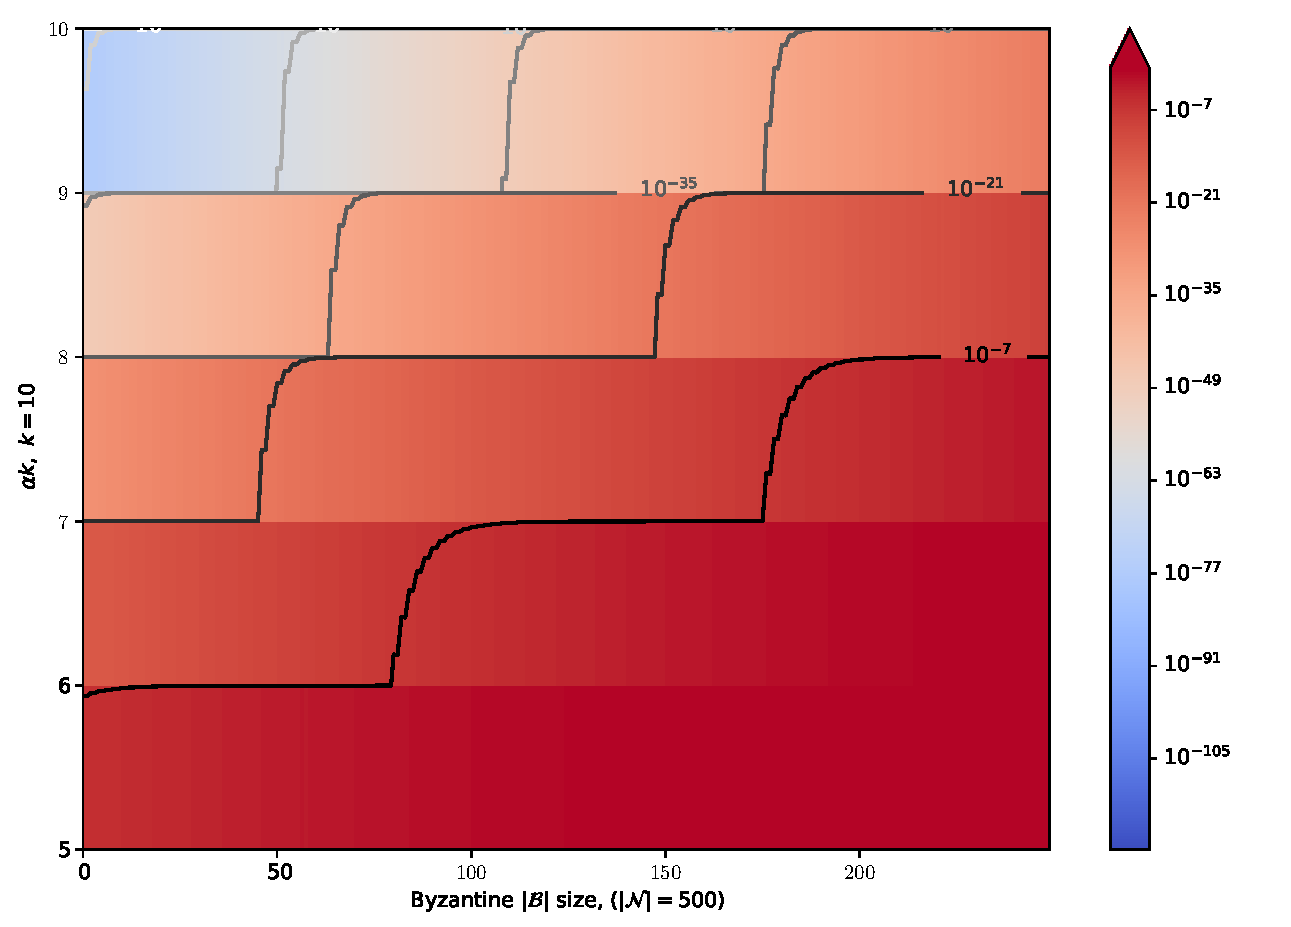
\includegraphics[width=\linewidth]{./figures/safety_failure.pdf}
\caption{Probability of safety failure, $\phi = 20$, $\delta = 100$, $|\mathcal{N}| = 500$, and $k = 10$, for various size of Byzantine nodes and $\alpha k$.}
\label{fig:safety_failure}
\end{figure}

% \subsubsection{Liveness of \Theta_1}
% A key metric related to liveness is convergence latency, the amount of time between the introduction of a value proposal to the time every correct node agress on the same value.
% Described in terms of network configurations, this convergence latency calculates the expected number of rounds from any bivalent network configuration until reaching a state where all correct nodes vote for the same value. 
% We first show that convergence latency for a Byzantine-free network is logarithmic in the size of the network. Later, we calculate bounds on the maximum adversarial size that still guarantees expected logarithmic convergence. 
% Let the system be initialized to state $\psi = \{|\mathcal{C}_1^{t_0}|, |\mathcal{C}_2^{t_0}|\}$. 
% We perform a Markovian analysis on the probabilities of transitioning to any of all the possible states arising from $\psi$. 
% The state space $\mathbb{S}$ of all possible configurations arising from $\psi$ is all possible bivalent network splits between values $1$ and $2$, such that $|\mathcal{C}_1^{t_0}| + |\mathcal{C}_2^{t_0}| = |\mathcal{N}|$. 
% As an example, suppose the total number of correct nodes is 100. Then, all possible states of the system are $\{0, 100\}, \{1, 99\}, \dots, \{100, 0\}$.
% We can now construct the transition probability matrix $M$ of size $|\mathbb{S}| \times |\mathbb{S}|$. The expression for generating the values inside $M$ is highly verbose, however to provide the reader some intuition on how it is build, we given an example. Suppose the system is at state $\{50, 50\}$. Then, the system can only move to states $\{49, 51\}$, $\{51, 49\}$, or itself. The probability of moving to $\{49, 51\}$ is the probability of selecting a node that votes value $2$ and having that node switch to value $1$. The probability of staying in place is the probability that any selected node does not achieve the required $\alpha k$ threshold, or it achieves a threshold for its own value. $M$ will be sparse since most states will have only a transition to a small number of states.

% Given any starting state $s \in \mathbb{S}$, the hitting time $\mu$ is the expected number of transitions to reach states $A = \{\{0, |C|\}, \{|C|, 0\}\}$. 
% To calculate the hitting time, we first construct the system of linear equations shown in equation \ref{equation:minimalsolution} for all states in $\mathbb{S}$.

% \begin{equation}
% \label{equation:minimalsolution}
% \begin{cases}
% \mu_{sA} = 0, & \forall s \in A\\
% \mu_{sA} = 1 +\sum_{r\notin A}^{}{p_{sr}\mu_{rA}}, & \forall s \notin A
% \end{cases}
% \end{equation}

% The minimal non-negative solution vector $\mu_{A}~=~(\mu_{sA}, s \in \mathbb{S})$ to the system of linear equations in equation \ref{equation:minimalsolution}, yields the expected number of rounds to reach one of the convergence states. In other words, the solution gives the expected number of rounds for each node before all nodes agree on the same value.

% The convergence latency grows logarithmically with the network size, as shown in Table \ref{table:growth_worst_case}. 
% At 10k nodes, for example, the equal-network split expected time to converge is around 10 rounds. 
% \begin{table}[h!]
% 	\centering
% 	\begin{tabular}{llllll}
% 		Net. Size   & 600    & 1200   & 2400   & 4800   & 9600    \\ \hline
% 		Exp. Conv. & 7.18 & 7.94 & 8.69 & 9.44 & 10.19
% 	\end{tabular}
% 	\caption{Expected number of per-node-iterations to convergence starting at worst-case (equal) network split. Network sizes grow exponentially, whereas worst-case convergence grows logarithmically. $k = 10,\ \alpha=6$.}
% 	\label{table:growth_worst_case}
% \end{table}

\paragraph{Adversarial Progress} 
Without loss of generality, let $\lambda$ be chosen such that the expected frequency of $v_1$ and $v_2$ amongst the $\lambda$ chosen neighbors is nearly the same as $cn(v_1)$ and $cn_(v_2)$. 
In order to prevent progress, the number of adversarial nodes must then be larger than the absolute difference between the total number of honest nodes that vote for $v_1$ and $v_2$. This absolute difference denotes the total number of nodes that the adversary must have in its control in order to maintain an equal split between honest nodes. This adversarial size denotes the minimal adversarial size to prevent convergence in expected logarithmic number of rounds. 

Conversely, we can look at the case when the adversary pushes honest nodes to commit one value, and then equivocates. In this case, As long as the adversary is greater than ($1 - \beta/\lambda$), honest nodes that have not yet committed will no longer be able to commit. Any and all solicitations from any honest node will result in expected $(\lambda-\beta)/\lambda$ or more equivocations, which is insufficient to make progress.

\label{section:analysis}
\subsection{Snowball Safety Analysis}
% \label{subsec:safetyanalysis}
% \subsubsection{Terminology and Definitions}
% \label{subsubsec:termanddef}
% In this subsection, we refresh the reader of some of the old notations and as well introduce new notation, terminology, and definitions. 
%Finally, let $T_i$ and $T_j$ be two conflicting transactions belonging to the same conflict set. 

In order to analyze the safety of our protocol, we turn our focus exclusively towards two transactions of interest, $T_i$ and $T_j$, which belong to the same conflict set. 
Although the system is comprised of many conflicting transactions, we can safely ignore transactions that are not in the ancestry or progeny sub-graph of $T_i$ and $T_j$, since -- by construction -- those transactions are completely independent from $T_i$ and $T_j$ and thus do not contribute to the evolution of preference for either of the transactions of interest. 
Lastly, we note that unless explicitly stated, the analysis is through a ``God's eye'' view of the network. 

In the specification section (S. \ref{subsection:specification}), we introduced the general definition of \textit{preference} for a transaction $T$. 
Using that definition, we construct the notion of \textit{network support} for $T$, denoted as $\mathcal{S}_{u}^{t}(T)$, which represents the fraction of nodes in $\mathcal{N}$ that prefer $T$ at time $t$ as perceived by node $u$. 
To illustrate, suppose that the correct nodes are equally split in preference between $T_i$ and $T_j$. Furthermore, let $\mathcal{B}_{u}^{t}(T_i), \mathcal{B}_{u}^{t}(T_j) \subseteq \mathcal{B}$, be the subsets of the Byzantine nodes that vote $T_i$ and $T_j$ respectively as perceived by node $u$, which are mutually exclusive since according to $u$'s perspective the same Byzantine node cannot prefer two equivocating transactions simultaneously. 
A correct node $u$ would then observe that the network support for $T_{\{i,j\}}$ must be $\mathcal{S}_{u}^{t}(T_{\{i,j\}}) = (|\mathcal{B}_{T_{\{i,j\}}}| + |\mathcal{C}|/2)/|\mathcal{N}|$). 

Lastly, we call a \textit{solicitation} the act of $u$ querying a set of $k$ neighbors, chosen uniformly at random, to discover if they prefer transaction $T_i$. 
Note that necessarily $k \leq |\mathcal{N}|$, but otherwise the choice of size of $k$ is independent of the size of $\mathcal{N}$, as discussed previously.

% \subsubsection{Network Model}
\paragraph{Network Model}
We initially assume that every node has full view of every other node. 
Later, we relax this requirement to allow for looser views. 
Each node maintains a logical round counter (time) that starts at 0 at its initial solicitation and is incremented by one for each solicitation of a child transaction. 
Importantly, we remind that there is no notion of global system rounds, unless explicitly stated.

For simplicity, we assume that each node receives all $k$ responses of a solicitation within the same round. 
Later, we relax this requirement to interleave solicitation responses. 

% \subsubsection{Byzantine Adversary}
% \label{subsec:byzantineadversary}
\paragraph{Byzantine Adversary}
The adversary, whose nodes are in set $\mathcal{B}$, is round-adaptive and can both read all messages and view the state of all nodes in the network.
Round-adaptive means that the adversary can choose a new strategy for each of its nodes after seeing the messages exchanged by correct nodes.
In other words, whenever a correct node solicits its neighbors, the adversary can correspondingly instruct nodes under its ownership before the correct node has the chance to receive any responses. 
Such an adversary is only prohibited from modifying the internal state of a correct node and the in-transit responses between any two correct nodes. 

\subsubsection{Analysis}
\label{subsec:analysis}
% \paragraph{Statistical Errors and Parameters}
% We begin the analysis by first extracting some statistical bounds on protocol parameters. 
% We extract these bounds by isolating a single correct node $u$, and analyzing the results of a single isolated network polling experiment. Basically, we freeze the network at some specific point in time $t$ and then compute the statistical errors between two nodes $u$ and $v$. 

% For notational ease, we represent $\mathcal{S}_{u}^{t}(T_i)$ as $\mathcal{S}'$. 
% Let $\mathcal{H}_{N, \mathcal{S}'}^k \rightarrow [0, k] \in \mathbb{N}$ be a random variable which represents the total count of the $k$ randomly chosen neighbors that prefer transaction $T_i$ at round $t$ as queried by $u$. $\mathcal{H}$ is parameterized by the sample size $k$, the network $\mathcal{N}$, and the network support of $T_i$, $\mathcal{S}'$. For some constant $1/2 \leq \alpha \leq 1$, we are interested in the probability that a majority or more, $\alpha k \in \mathbb{N}$, of the sampled $k$ neighbors prefer $T_i$. The probability can be calculated as follows, 
% \begin{equation}
% P(\mathcal{H}_{\mathcal{N}, \mathcal{S}'}^k \geq \alpha k) = \sum_{j = \alpha k}^{k} \frac{{\mathcal{S}'|\mathcal{N}| \choose j}{|\mathcal{N}| - \mathcal{S}'|\mathcal{N}| \choose k - j}}{{|\mathcal{N}| \choose k}}
% \label{eq:hypergeometric}
% \end{equation}
% where the expected value of $\mathcal{H}_{\mathcal{N}, \mathcal{S}'}^k$ is exactly $k\mathcal{S}'$. From now on, if $\mathcal{H}_{N, \mathcal{S}'}^k \geq \alpha k$, we say that the solicitation was successful. 
% %Intuitively, the meaning behind this term is that some threshold majority $\alpha k$ of the solicited neighbors indeed support the transaction in question.

% We use the Hoeffding \cite{hoeffding1963probability} inequality to calculate the probabilities of deviation from the expected result of the polling experiment. Hoeffding's tail bounds then show that -- given a fixed constant $\psi$ -- the probability $\mathcal{H}$ deviating by $\psi$ from the expected value is given by, 
% \begin{equation}
% \begin{split}
%     P(\mathcal{H}_{N, \mathcal{S}'}^k \leq (\mathcal{S}'-\psi)k) %&\leq e^{-k\mathcal{D}(\mathcal{S}'-\psi, \mathcal{S}')} %\\
%     %&
%     \leq e^{-2\psi^2k}
% \end{split}
% \end{equation}
% % where $\mathcal{D}(\mathcal{S}'-\psi, \mathcal{S}')$ is the Kullback-Leibler divergence, measured as
% % \begin{equation}
% % \begin{split}
% %     \mathcal{D}(\mathcal{S}'-\psi, \mathcal{S}') &= (\mathcal{S}'-\psi) \log (\frac{\mathcal{S}'-\psi}{\mathcal{S}'}) \\
% %     &+ (1 - \mathcal{S}' + \psi) \log \frac{1 - \mathcal{S}' + \psi}{1 - \mathcal{S}'}
% % \end{split}
% % \end{equation}
% The very first thing to notice is that the probabilities are independent of network size, meaning that network size doesn't affect the performance of the protocol. 

% The second thing to notice is that the the upper bound $e^{-2\psi^2k}$ indicates that the probability of success of a solicitation is an inverse exponential parametrized by the sample size $k$. 
% For $k$, every +1 increase means an \textit{exponential decrease} in network view error.

% The third and last thing to notice is the implication for the value $\psi$, which has a quadratic effect on the exponential decrease in network view error. The network split amongst the correct nodes that maximizes the tail bound probability is exactly when half of the correct nodes are partitioned to initially prefer $T_i$ and half to initially prefer $T_j$. If the Byzantine nodes partition the network at some other ratio, the probability the Byzantine adversary successfully forces $u$ to prefer $T_i$ and $v$ to prefer $T_j$ for one solicitation is suboptimal. However, although this conclusion is correct over a single polling experiment, it may not hold over multiple experiments. This is because it would need to account for changes in the underlying graph structure. To that end, we now begin to analyze the protocol as it evolves over time. 

% % The implication of this result is that the optimal strategy for the Byzantine nodes is to minimize the deviation of $\psi$ (i.e. $\psi, k \rightarrow 0$), by splitting the network equally into two conflicting halves. 

% %The structure of the dag confers an important property. 
% %Due to the invariant imposed by the structure of the dag which states that every transaction on the path to a preferred child must be preferred in turn, every successful solicitation of a transaction implies a successful solicitation of its parent. 
% % Let $T' \xleftarrow{*} T$. At any time $t$, we necessarily have 
% % \begin{equation}
% % P(\mathcal{H}_{N, \mathcal{S}_{u}^{t}(T')}^k \geq \alpha k) \geq P(\mathcal{H}_{N, \mathcal{S}_{u}^{t}(T)}^k \geq \alpha k)
% % \end{equation}
% % We can now substitute the net total solicitations of the child transactions with an equivalent set of repeated solicitations for the parent transaction. 
% % This simplification allows us to focus solely on $T_i$, and safely ignore all other transactions except direct ancestors of $T_i$. 

% % Let $\mathcal{P}_b$ = $\{T_i, T_j\}$ be a set of two conflicting transactions. 
% % Let $u, v \in \mathcal{C}$ be any two correct nodes, and let $c_{\{u, v\}}(T_{\{i,j\}}, n)$ represent the confidence (i.e. the number of successful solicitations) for each of the transactions by each of the two correct nodes after sampling $n$ children transactions at rounds $t_0, t_1, \dots, t_n$, respectively. 

% % The expectation of the confidence of transaction $T_i$ after $n$ solicitations is equal to the probability of a successful solicitation for $T_i$ summed independently over every one of the $n$ experiments. More precisely, 
% % \begin{equation}
% % \begin{split}
% %     \mathbb{E}[c_{u}(T_{i}, n)] &=\ \sum_{j = 0}^{n}P(\mathcal{H}_{N, \mathcal{S}_{u}^{t_j}(T_i)}^k \geq \alpha k) \\
% % \end{split}
% % \end{equation}
\paragraph{Evolution Over Time}
The Byzantine nodes have the freedom to attack the system using any strategy. 
In order to maximize damage, the Byzantine nodes must pick the path of execution that ensures that the confidence of the two equivocating transactions is maximized between two correct nodes.
The adversary has access to a large set of attack options. On the one extreme end, the adversary may launch a ``bifurcation attack'', where the attacker equivocates at the very beginning and attempts to split the network equally in half, hoping that part of the network slowly prefers one transaction and the other half prefers the other. On the other extreme end, the adversary can launch a ``double-spend'' attack, where the adversary behaves correctly at the beginning, but after some large amount of time equivocates. 

% To calculate these expectations, and consequently define the most damaging Byzantine strategy, we must first extract some tail bounds on $\mathcal{H}$. 
%Figure \ref{fig:hypersplits} shows the probability of a single successful experiment over various network splits. 
%The probability of a single successful iteration decreases poly-exponentially with increasing difference between $\mathcal{S}N$ and $\alpha k$. 
% The most relevant tail bound can be extracted from Hoeffding \cite{hoeffding1963probability}. Given a network support $\mathcal{S}'$, the expected value of $\mathcal{H}_{N, \mathcal{S}'}^k$ is exactly $k \mathcal{S}'$. Hoeffding's inequality then shows that -- given a fixed constant $\psi$ -- the probability $\mathcal{H}$ deviating by $\psi$ from the expected value is given by, 
% \begin{equation}
% \begin{split}
%     P(\mathcal{H}_{N, \mathcal{S}'}^k \leq (\mathcal{S}'-\psi)k) %&\leq e^{-k\mathcal{D}(\mathcal{S}'-\psi, \mathcal{S}')} %\\
%     %&
%     \leq e^{-2\psi^2k}
% \end{split}
% \end{equation}
% % where $\mathcal{D}(\mathcal{S}'-\psi, \mathcal{S}')$ is the Kullback-Leibler divergence, measured as
% % \begin{equation}
% % \begin{split}
% %     \mathcal{D}(\mathcal{S}'-\psi, \mathcal{S}') &= (\mathcal{S}'-\psi) \log (\frac{\mathcal{S}'-\psi}{\mathcal{S}'}) \\
% %     &+ (1 - \mathcal{S}' + \psi) \log \frac{1 - \mathcal{S}' + \psi}{1 - \mathcal{S}'}
% % \end{split}
% % \end{equation}
% The very first thing to notice is that the probabilities are independent of network size, and are only a function of the sampled neighbor size $k$. This means that the network size doesn't affect performance of the protocol.

% The second thing to notice is that the the upper bound $e^{-2\psi^2k}$ indicates that the probability of success of a solicitation is an inverse exponential parametrized by the squared value of $\psi$. 
% The implication of this result is that the optimal strategy for the Byzantine nodes is to minimize the deviation of $\psi$ (i.e. $\psi, k \rightarrow 0$), by splitting the network equally into two conflicting halves. 
%Correct nodes can be fooled by Byzantine nodes by tuning parameters such that $e^{-2\psi^2k}$ is maximized. 
%This occurs when the deviation and sample size approach zero (i.e. $\psi, k \rightarrow 0$). 
% Since the Byzantine nodes are limited in their network presence, the most damaging strategy must necessarily be when all correct nodes are equally split. 

We start calculating the evolution of confidence between $T_i$ and $T_j$ by first computing the network split between the two transactions without introducing any children transactions. Let $T_*$.\texttt{sum} be the total sum of all chits for transaction $T_*$ amongst all correct nodes in the network. Let $\mathcal{C}_1$ be the subset of correct nodes that prefer $T_i$ at time $t = 0$, and $\mathcal{C}_2$ the corresponding set for $T_j$. Lastly, let $\mathcal{Z}_1$ be the subset of correct nodes that the Byzantine nodes have chosen to force to prefer $T_i$, and $\mathcal{Z}_2$ be the corresponding set of nodes for $T_j$. At $t = 1$ (the base case), the we can compute the new values of $T_*$.\texttt{sum} as follows:

\begin{equation}
    \begin{split}
        & T_1.\text{\texttt{sum}} = 0;\ T_2.\text{\texttt{sum}} = 0;\\
        t_1:\ \ \ &\gamma_{1}^{t_1} \leftarrow \frac{\mathcal{Z}_1}{\mathcal{C}} P(\mathcal{H}(\mathcal{N}, \mathcal{C}_1 + \mathcal{B}, k, \alpha) \geq \alpha k)
        % = \sum_{i = \alpha}^{k} {k \choose i}\bigg(\frac{\mathcal{C}_1 + \mathcal{B}}{\mathcal{N}}\bigg)^i \bigg(1 - \frac{\mathcal{C}_1 + \mathcal{B}}{\mathcal{N}}\bigg)^{k - i}
        \\
        & \gamma_{2}^{t_1} \leftarrow \frac{\mathcal{Z}_2}{\mathcal{C}} P(\mathcal{H}(\mathcal{N}, \mathcal{C}_1, k, \alpha) \geq \alpha k) 
        %= \sum_{i = \alpha}^{k} {k \choose i}\bigg(\frac{\mathcal{C}_1}{\mathcal{N}}\bigg)^i \bigg(1 - \frac{\mathcal{C}_1}{\mathcal{N}}\bigg)^{k - i}
        \\
        & T_1.\text{\texttt{sum}} = T_1.\text{\texttt{sum}} + \gamma_{1}^{t_1} + \gamma_{2}^{t_1}\\
        &\xi_{1}^{t_1} \leftarrow \frac{\mathcal{Z}_1}{\mathcal{C}} P(\mathcal{H}(\mathcal{N}, \mathcal{C}_2, k, \alpha) \geq \alpha k)\\
        & \xi_{2}^{t_1} \leftarrow \frac{\mathcal{Z}_2}{\mathcal{C}} P(\mathcal{H}(\mathcal{N}, \mathcal{C}_2 + \mathcal{B}, k, \alpha) \geq \alpha k)\\
        & T_2.\text{\texttt{sum}} = T_2.\text{\texttt{sum}} + \xi_{1}^{t_1} + \xi_{2}^{t_1}\\
    \end{split}
\end{equation}

In other words, the new expected value of $T_1$.\texttt{sum} after a single time-step is the probability that a correct node in $\mathcal{Z}_1$ is chosen and that node successfully samples at least $\alpha k$ neighbors that also prefer $T_i$ plus the probability that a correct node in $\mathcal{Z}_2$ is chosen and that node successfully samples at least $\alpha k$ neighbors that also prefer $T_i$. In the next time-step, we must include the newly-updated transaction preference sums as part of the computation. For the rest of the time-steps, we compute as follows:

\begin{equation}
    \begin{split}
        t_2:\ \ \ &\gamma_{1}^{t_2} \leftarrow \frac{\mathcal{Z}_1}{\mathcal{C}} P(\mathcal{H}(\mathcal{N}, \mathcal{C}_1 + \mathcal{B} + \gamma_{2}^{t_1} - \xi_{1}^{t_1}, k, \alpha) \\&\geq \alpha k)\\
        & \gamma_{2}^{t_2} \leftarrow \frac{\mathcal{Z}_2}{\mathcal{C}} P(\mathcal{H}(\mathcal{N}, \mathcal{C}_1 + \gamma_{2}^{t_1} - \xi_{1}^{t_1}, k, \alpha) \geq \alpha k)\\
        & T_1.\text{\texttt{sum}} = T_1.\text{\texttt{sum}} + \gamma_{1}^{t_2} + \gamma_{2}^{t_2}\\
        &\xi_{1}^{t_2} \leftarrow \frac{\mathcal{Z}_1}{\mathcal{C}} P(\mathcal{H}(\mathcal{N}, \mathcal{C}_2 + \xi_{1}^{t_1} - \gamma_{2}^{t_1}, k, \alpha) \geq \alpha k)\\
        & \xi_{2}^{t_2} \leftarrow \frac{\mathcal{Z}_2}{\mathcal{C}} P(\mathcal{H}(\mathcal{N}, \mathcal{C}_2 + \mathcal{B} + \xi_{1}^{t_1} - \gamma_{2}^{t_1}, k, \alpha) \geq \alpha k)\\
        & T_2.\text{\texttt{sum}} = T_2.\text{\texttt{sum}} + \xi_{1}^{t_2} + \xi_{2}^{t_2}\\
        t_3:\ \ \ &\gamma_{1}^{t_3} \leftarrow \frac{\mathcal{Z}_1}{\mathcal{C}} P(\mathcal{H}(\mathcal{N}, \mathcal{C}_1 + \mathcal{B} + \gamma_{2}^{t_1} + \gamma_{2}^{t_2} - \xi_{1}^{t_1} - \xi_{1}^{t_2}, k, \alpha) \geq \alpha k)\\
        & \gamma_{2}^{t_3} \leftarrow \frac{\mathcal{Z}_2}{\mathcal{C}} P(\mathcal{H}(\mathcal{N}, \mathcal{C}_1  + \gamma_{2}^{t_1} + \gamma_{2}^{t_2} - \xi_{1}^{t_1} - \xi_{1}^{t_2}, k, \alpha) \geq \alpha k)\\
        & T_1.\text{\texttt{sum}} = T_1.\text{\texttt{sum}} + \gamma_{1}^{t_3} + \gamma_{2}^{t_3}\\
        &\xi_{1}^{t_3} \leftarrow \frac{\mathcal{Z}_1}{\mathcal{C}} P(\mathcal{H}(\mathcal{N}, \mathcal{C}_2 + \xi_{1}^{t_1} + \xi_{1}^{t_2} - \gamma_{2}^{t_1} - \gamma_{2}^{t_2}, k, \alpha) \geq \alpha k)\\
        & \xi_{2}^{t_3} \leftarrow \frac{\mathcal{Z}_2}{\mathcal{C}} P(\mathcal{H}(\mathcal{N}, \mathcal{C}_2 + \mathcal{B} + \xi_{1}^{t_1} + \xi_{1}^{t_2} - \gamma_{2}^{t_1} - \gamma_{2}^{t_2}, k, \alpha) \geq \alpha k)\\
        & T_2.\text{\texttt{sum}} = T_2.\text{\texttt{sum}} + \xi_{1}^{t_3} + \xi_{2}^{t_3}\\
        t_4:\ \ \ & \dots
    \end{split}
\end{equation}

Calculating this complex expression, we arrive at the following results shown in Figures \ref{fig:variousalpha}, \ref{fig:variousk}, and \ref{fig:variousb}.

\begin{figure}[h!]
\centering
\includegraphics[width=\linewidth]{./various_alpha.png}
\caption{Various $\alpha$}
\label{fig:variousalpha}
\end{figure}

\begin{figure}[h!]
\centering
\includegraphics[width=\linewidth]{./various_k.png}
\caption{Various $k$}
\label{fig:variousk}
\end{figure}

\begin{figure}[h!]
\centering
\includegraphics[width=\linewidth]{./various_b.png}
\caption{Various $\mathcal{B}$}
\label{fig:variousb}
\end{figure}

$<<$TODO: DISCUSS IMPLICATIONS OF THE GRAPH, AND HOW THEY SUPPORT PRIOR CLAIMS.$>>$

At $t_0$, the Byzantine nodes partitioned the correct nodes according to some strategy, and we computed the expected outcomes of the network preferences after all correct nodes had a chance to poll. We now continue computing the evolution of the preferences in the network by introducing children transactions. For simplicity, we first assume that the children transactions all belong to partitions of size one, even if the children transactions are generated by Byzantine nodes.

Due to the invariant imposed by the structure of the dag which states that every transaction on the path to a preferred child must be preferred in turn, every successful solicitation of a transaction implies a successful solicitation of its parent. Moreover, and more importantly, the network support for every immediate child transaction is exactly equal to the probability of the parent being preferred. 
Let $T' \xleftarrow{} T$. At any time $t$, we necessarily have 
\begin{equation}
P(\mathcal{H}_{N, \mathcal{S}_{u}^{t}(T')}^k \geq \alpha k) \geq P(\mathcal{H}_{N, \mathcal{S}_{u}^{t}(T)}^k \geq \alpha k)
\end{equation}
and, more importantly, the 
\begin{equation}
\mathcal{S}_{u}^{t_b}(T) = \mathbb{E}[\mathcal{H}_{N, \mathcal{S}_{u}^{t_a}(T')}^k]/k
\end{equation}
where $t_b$ is larger than $t_a$. 
The expectation of confidence between two conflicting transaction in a permanently split network after $n$ rounds is then
\begin{equation}
    \begin{split}
        \mathbb{E}[c_{u}(T_{i}, n)] &=\ \mathbb{E}[c_{v}(T_{j}, n)]\\
         &=\ nP(\mathcal{H}_{\mathcal{N}, |\mathcal{H}|/2 + |\mathcal{B}|}^k \geq \alpha k)\\
\end{split}
\end{equation}

Before moving on, we can now extract some numerical values. 
Let $|\mathcal{N}| = 10000$, where 25\% of nodes are Byzantine.
Let half of the correct nodes prefer $T_i$ such that $d(T_i) = 1$ and $d(T_j) = 0$, and the other half prefer $T_j$ such that $d(T_i) = 0$ and $d(T_j) = 1$.
Let $u$ be a correct node that prefers $T_i$ and $v$ a correct node that prefers $T_j$.
Let $\alpha k$ = 180, and $k$ = 200. 
Then, 
\begin{equation}
    \begin{split}
    P(\mathcal{H}_{\mathcal{N}, \mathcal{S}_{u}^{t_1}(T_i)}^k \geq \alpha k) &= P(\mathcal{H}_{\mathcal{N}, \mathcal{S}_{v}^{t_1}(T_j)}^k \geq \alpha k)\\
    &= 5.616\times10^{-19}
    \end{split}
\end{equation}
as calculated from equation \ref{eq:hypergeometric}. 
If compounded over all nodes in the network, then the probability that any two nodes from the two preferrence subsets successfully increase confidence in their respective preference is $4.435\times10^{-30}$. 
% Other splits are shown in Figure \ref{fig:hypersplits}. 
%The probability that specifically $u$ and $v$ prefer $T_i$ and $T_j$ for only a preference difference of 1 is $3.154\times10^{-37}$. 
%If we compound over all pairs of partitioned correct nodes, then the probability increases to $4.435\times10^{-30}$. 
Notice that this is for a single round. If we assume a throughput of 1000 solicitations/second, then the probability of success over a second increases to $4.435\times10^{-27}$. Therefore, the expected time before any two correct nodes prefer two equivocating transactions can be calculated through the mean of the geometric distribution and is equal to $2.25\times10^{26}$ seconds, or about $7.14\times10^{18}$ years.

Notice that the calculation above is the optimal probability. Other splits in network result in far lower probabilities and far longer times. Furthermore, notice that the above Byzantine attack assumes that Byzantine nodes can arbitrarily generate transactions \textit{at will}. In reality, simple anti-transaction-flooding measures would severely cripple the Byzantine adversary. 

Let's break down the intuition of the results in our analysis. 
The tail bounds indicate that as long as a reasonably large $k$ sample size is picked, the only way for the Byzantine nodes to fool any correct node is to actually build enough network confidence for the transaction. 
The threshold $\alpha$ can be chosen as a function of the Byzantine size, where the higher the Byzantine presence, the larger the threshold should be set. 

The consequence of a higher $\alpha$, however, is that it is possible for the Byzantine nodes to deny service to the network. Since liveness is decoupled from safety, we later introduce non-protocol specific mechanisms to thwart such behavior, ensuring that rogue transactions die out quickly and virtuous transactions get accepted quickly.

\subsubsection{Network View}
The analysis up to now assumes that the network view is fully consistent among all nodes. 
In any real open distributed system, such an assumption invariably breaks downs. 
Therefore, we must quantify the amount of tolerance in network view discrepancy between any two correct nodes. 

Safety may be violated using a subnetwork partition attack. 
The Byzantine nodes are able to partition the network into several subnetworks such that each subnetwork shares only some set of correct nodes. 
To make this clear, let $\mathcal{E}_{1}, \mathcal{E}_{2} \subset \mathcal{N}$, where $\mathcal{E}_1 \cup \mathcal{E}_2 = \mathcal{N}$, be two subsets of the entire network of nodes, where all members of each subset have -- at minimum -- all other members in the same subset in their view. 
Lastly, let the nodes in the intersection $\mathcal{E}_1 \cap \mathcal{E}_2$ have a view of all nodes in $\mathcal{E}_1$ and $\mathcal{E}_2$. 
We can then view each subnetwork independently of each other, and apply the same analysis as before. The difference, however, is that the network of nodes from the perspective of each subnetwork is not $\mathcal{N}$, but rather just $\mathcal{E}_*$. Therefore, if the Byzantine presence with a fully consistent view was only $\mathcal{B}/\mathcal{N}$, it now becomes $\mathcal{B}/\mathcal{E}_*$. In the worst case scenario, if $|\mathcal{E}_1 \cap \mathcal{E}_2| < (k - \alpha k)$, then safety can be violated without any Byzantine presence. However, in practice, although churn exists, such large network partition is difficult to achieve. 

In later sections, we introduce the Snowball network overlay protocol, which guarantees with high probability that the network doesn't suffer from large partitioning. 

% \begin{figure}
% \centering
% \includegraphics[width=\linewidth]{./hypersplits.pdf}
% \caption{Probability of single successful sample over different network splits.}
% \label{fig:hypersplits}
% \end{figure}
\end{comment}
